
\chapter{Git}

%% link to git cheatsheet
\href{https://training.github.com/downloads/github-git-cheat-sheet.pdf}{GitHub Cheatsheet}

\section{About Git}

\subsection{About version control and Git}

\begin{definitionblock}[Version control]
    A version control system, or VCS, tracks the history of changes as people and teams collaborate on projects together. As developers make changes to the project, any earlier version of the project can be recovered at any time.
\end{definitionblock}

Developers can revew project history to find out:
\begin{itemize}
    \item Which changes were made?
    \item Who made the changes?
    \item When were the changes made?
    \item Why were changes needed?
\end{itemize}

In a \textbf{distributed version control system (DVCSs)}, every developer has a full copy of the prokect and project history. They don't need a constant connection to a central repository. \texttt{Git} is the most popular distributed version control syste. It is commonly used for both open source and commercial software development, with significant benefits for individuals, teams and businesses. 

\begin{tipsblock}
    \begin{itemize}
        \item \textbf{Git lens} is used to see the entire timeline of the project, including decisions, changes and progressions. From the moment they access the history of a project, the developer has all the context they need to understand it and start contributing.
        \item Developers work in every time zone. With a DVCS like Git, collaboration can happen any time while maintaining source code integrity. Using \textbf{branches}, developers can safely propose changes to production code.
    \end{itemize}
\end{tipsblock}

\subsection{Repositories}

A repository, or Git project, encompasses the entire collection of files and folders associated with a project, along with each file's revision history. The file history appears as \textbf{snapshots} in time called commits. The commits can be organized into multiple lines of development called branches. Because Git is a DVCS, repositories are self-contained units and anyone who has a copy of the repository can access the entire codebase and its history. Using the command line or other ease-of-use interfaces, a Git repository also allows for: interaction with the history, cloning the repository, creating branches, committing, merging, comparing changes across versions of code, and more.

A repository, or Git project, encompasses the entire collection of files and folders associated with a project, along with each file's revision history. The file history appears as snapshots in time called commits. The commits can be organized into multiple lines of development called branches. Because Git is a DVCS, repositories are self-contained units and anyone who has a copy of the repository can access the entire codebase and its history. Using the command line or other ease-of-use interfaces, a Git repository also allows for: interaction with the history, cloning the repository, creating branches, committing, merging, comparing changes across versions of code, and more.

\subsection{GitHub}

GitHub hosts Git repositories and provides developers with tools to ship better code through command line features, issues (threaded discussions), pull requests, code review, or the use of a collection of free and for-purchase apps in the GitHub Marketplace. With collaboration layers like the GitHub flow, a community of 100 million developers, and an ecosystem with hundreds of integrations, GitHub changes the way software is built.

GitHub builds collaboration directly into the development process. Work is organized into repositories where developers can outline requirements or direction and set expectations for team members. Then, using the GitHub flow, developers simply create a branch to work on updates, commit changes to save them, open a pull request to propose and discuss changes, and merge pull requests once everyone is on the same page. 

\subsection{Command Line Interface}

To use Git, developers use specific commands to copy, create, change, and combine code. These commands can be executed directly from the command line or by using an application like GitHub Desktop. Here are some common commands for using Git:

\begin{itemize}
    \item \texttt{git init}: Initializes a new Git repository. Until you run this command inside a repository or directory, it's just a regular folder. Only after you input this does it accept further Git commands.
    \item \texttt{git config}: Short for "configure," this is most useful when you're setting up Git for the first time.
    \item \texttt{git help}: Forgot a command? Type this into the command line to bring up the 21 most common git commands.
    \item \texttt{git status}: We all get a little nervous the first time we commit our changes. This command shows you the status of changes as untracked, modified, or staged.
    \item \texttt{git add}: This does not add new files to your repository. Instead, it brings new files to Git's attention. After you add files, they're included in Git's "snapshots" of the repository.
    \item \texttt{git commit}: Git's most important command. After you make any sort of change, you input this in order to take a "snapshot" of the repository. Usually it goes \texttt{git commit -m "Message here"}.
    \item \texttt{git branch}: Working on multiple features at once? Use this command to list, create, or delete branches.
    \item \texttt{git checkout}: Literally allows you to "check out" a repository that you are not currently inside. This is a navigational command that lets you move to the repository you want to check.
    \item \texttt{git merge}: When you're done working on a branch, you can merge your changes back to the master branch, which is visible to all collaborators.
    \item \texttt{git push}: If you're working on your local computer, and want your commits to be visible online on GitHub as well, you "push" the changes up to GitHub with this command.
    \item \texttt{git pull}: If you're working on your local computer and want your commits to be visible online on GitHub as well, you "push" the changes up to GitHub with this command.
    \item \texttt{git clone}: If you're starting fresh and want to clone an existing repository from GitHub to your local computer, you can use this command to copy the repository to your computer.
    \item \texttt{git remote}: When you clone a repository from GitHub, it automatically creates a connection or "remote" that you can also push changes to.
\end{itemize}

\textbf{\\ Example: Contribute to an existing repository}
\begin{codeblock}[language=bash]
# download a repository on GitHub to our machine
# Replace `owner/repo` with the owner and name of the repository to clone
git clone https://github.com/owner/repo.git

# change into the `repo` directory
cd repo

# create a new branch to store any new changes
git branch my-branch

# switch to that branch (line of development)
git checkout my-branch

# make changes, for example, edit `file1.md` and `file2.md` using the text editor

# stage the changed files
git add file1.md file2.md

# take a snapshot of the staging area (anything that's been added)
git commit -m "my snapshot"

# push changes to github
git push --set-upstream origin my-branch
\end{codeblock}

\textbf{\\ Example: Start a new repository adn publish on GitHub}
\begin{codeblock}[language=bash]
# create a new directory, and initialize it with git-specific functions
git init my-repo

# change into the `my-repo` directory
cd my-repo

# create the first file in the project
touch README.md

# git isn't aware of the file, stage it
git add README.md

# take a snapshot of the staging area
git commit -m "add README to initial commit"

# provide the path for the repository you created on github
git remote add origin https://github.com/YOUR-USERNAME/YOUR-REPOSITORY-NAME.git

# push changes to github
git push --set-upstream origin main
\end{codeblock}

\textbf{\\ Example: Contribute to an existing branch on GitHub}
\begin{codeblock}[language=bash]
# change into the `repo` directory
cd repo

# update all remote tracking branches, and the currently checked out branch
git pull

# change into the existing branch called `feature-a`
git checkout feature-a

# make changes, for example, edit `file1.md` using the text editor

# stage the changed file
git add file1.md

# take a snapshot of the staging area
git commit -m "edit file1"

# push changes to github
git push
\end{codeblock}

\subsection{Models for collaborative development}

THere are two primary ways people collaborate on GitHub:
\begin{itemize}
    \item \textbf{Fork and pull model}: A project owner creates a master repository, and contributors fork that repository to their accounts. They clone the repository to their local machine, make changes, commit them
    \item \textbf{Shared repository model}: In this model, all collaborators have push access to the same repository. This is more common for small teams and organizations.
\end{itemize}

With a shared repository, individuals and teams are explicitly designated as contributors with read, write, or administrator access. This simple permission structure, combined with features like protected branches, helps teams progress quickly when they adopt GitHub.

For an open source project, or for projects to which anyone can contribute, managing individual permissions can be challenging, but a fork and pull model allows anyone who can view the project to contribute. A fork is a copy of a project under a developer's personal account. Every developer has full control of their fork and is free to implement a fix or a new feature. Work completed in forks is either kept separate, or is surfaced back to the original project via a pull request. There, maintainers can review the suggested changes before they're merged. 

\newpage
\section{Pushing commits to a remote repository}

\subsection{About \texttt{git push}}

The \texttt{git push} command takes two arguments.
\begin{itemize}
    \item A remote name, for example, \texttt{origin}
    \item A branch name, for example, \texttt{main}
\end{itemize}

For example, the command \texttt{git push origin main} pushes the commits in the local \texttt{main} branch to the remote repository named \texttt{origin}.
\begin{exampleblock}[Pushing changes to a remote repository]
    \begin{codeblock}[language=bash]
# push changes to the remote repository
git push origin main
    \end{codeblock}
\end{exampleblock}

\subsection{Renaming branches}

To rename a branch, you'd use the same \texttt{git push} command, but you would add one more argument: the name of the new branch. For example:
\begin{exampleblock}[Renaming a branch]
    \begin{codeblock}[language=bash]
# rename the local branch to new-name
git push origin main:new-name
    \end{codeblock}
\end{exampleblock}

This pushes the \texttt{main} branch to the remote repository, but the branch is renamed to \texttt{new-name}.
\begin{tipsblock}
    \begin{itemize}
        \item If you want to delete a branch, you can use the \texttt{--delete} flag with the \texttt{git push} command. For example, \texttt{git push origin --delete new-name} will delete the \texttt{new-name} branch from the remote repository.
        \item If you want to rename the branch you're currently on, you can use the \texttt{-u} flag to set the upstream branch. For example, \texttt{git push -u origin main:new-name} will push the \texttt{main} branch to the remote repository, renaming it to \texttt{new-name}, and set the upstream branch to \texttt{new-name}.
    \end{itemize}
\end{tipsblock}

\newpage
\subsection{Dealing with "non-fast-forward" errors}

If your local copy of a repository is out of sync with, or "behind", the upstream repository you're pushing to, you'll get a message saying \texttt{non-fast-forware updates were rejected}. This means that you must retrieve, or "fetch," the upstream changes, before you are able to push your local changes.

\begin{tipsblock}[Fetching]
    Fetching means retrieving recent commits from a remote repository without merging them into your local branch. This lets you view and compare new changes before deciding how to incorporate them into your work.
\end{tipsblock}

To fetch the changes from the remote repository, you can use the \texttt{git fetch} command. This command retrieves the changes from the remote repository, but it doesn't merge them into your local branch. After fetching the changes, you can merge them into your local branch using the \texttt{git merge} command.

\subsection{Pushing tags}

By default, and without additional parameters, \texttt{git push} sends all matching branches that have the same names as remote branches. 

To push a single tag, you cna issue the same command as pushing a branch:
\begin{codeblock}[language=bash]
git push origin tag-name
\end{codeblock}

To push all your tags, you can type the command:
\begin{codeblock}[language=bash]
git push origin --tags
\end{codeblock}

\subsection{Deleting a remote branch or tag}

The syntax to delete a branch is a bit more arcane at first glance:
\begin{codeblock}[language=bash]
git push origin --delete branch-name
\end{codeblock}

Note that there is a space before the colon. The command resembles the same steps you'd take to rename a branch. However, here, you're telling Git to push \textbf{nothing} into \texttt{branch-name}, effectively deleting it. Because of this, \texttt{git push} deletes the branch on the remote repository. 

\subsection{Remotes and forks}

You can \textbf{fork a repository} on GitHub. 

When you clone a repository you own, you provide it with a remote URL that tells Git where to fetch and push updates. If you want to collaborate with the original repository, you'd add a new remote URL, typically called \texttt{upstream}, to your local Git clone:
\begin{codeblock}[language=bash]
git remote add upstream REMOTE_URL 
\end{codeblock}

Now you can fetch updates and branches from their fork:
\begin{codeblock}[language=bash]
git fetch upstream
# Grab the upstream remote's branches
> remote: Counting objects: 75, done.
> remote: Compressing objects: 100% (53/53), done.
> remote: Total 62 (delta 27), reused 44 (delta 9)
> Unpacking objects: 100% (62/62), done.
> From https://github.com/OCTOCAT/REPO
>  * [new branch]      main     -> upstream/main
\end{codeblock}

When you're done making local changes, you can push your local branch to GitHub and initiate a pull request. 

\section{Getting changes from a remote repository}

\subsection{Options for getting changes}
These commands are very useful when interacting with a remote repository. \texttt{clone} and \texttt{fetch} download remote code from a repository's remote URL to your local computer, \texttt{merge} is used to merge different people's work together with yours, and \texttt{pull} is a combination of \texttt{fetch} and \texttt{merge}.

\subsection{Cloning a repository}
To grab a complete copy of another user's repository, use \texttt{git clone} like this:
\begin{codeblock}[language=bash]    
git clone https://github.com/USERNAME/REPOSITORY.git 
# Clones a repository to your computer
\end{codeblock}

You can choose from different URLs when cloning a repository. While logged in to GitHub, there URLs are available on the main page of the repository when you click \texttt{<> Code}.

\begin{figure}[H]
    \centering
    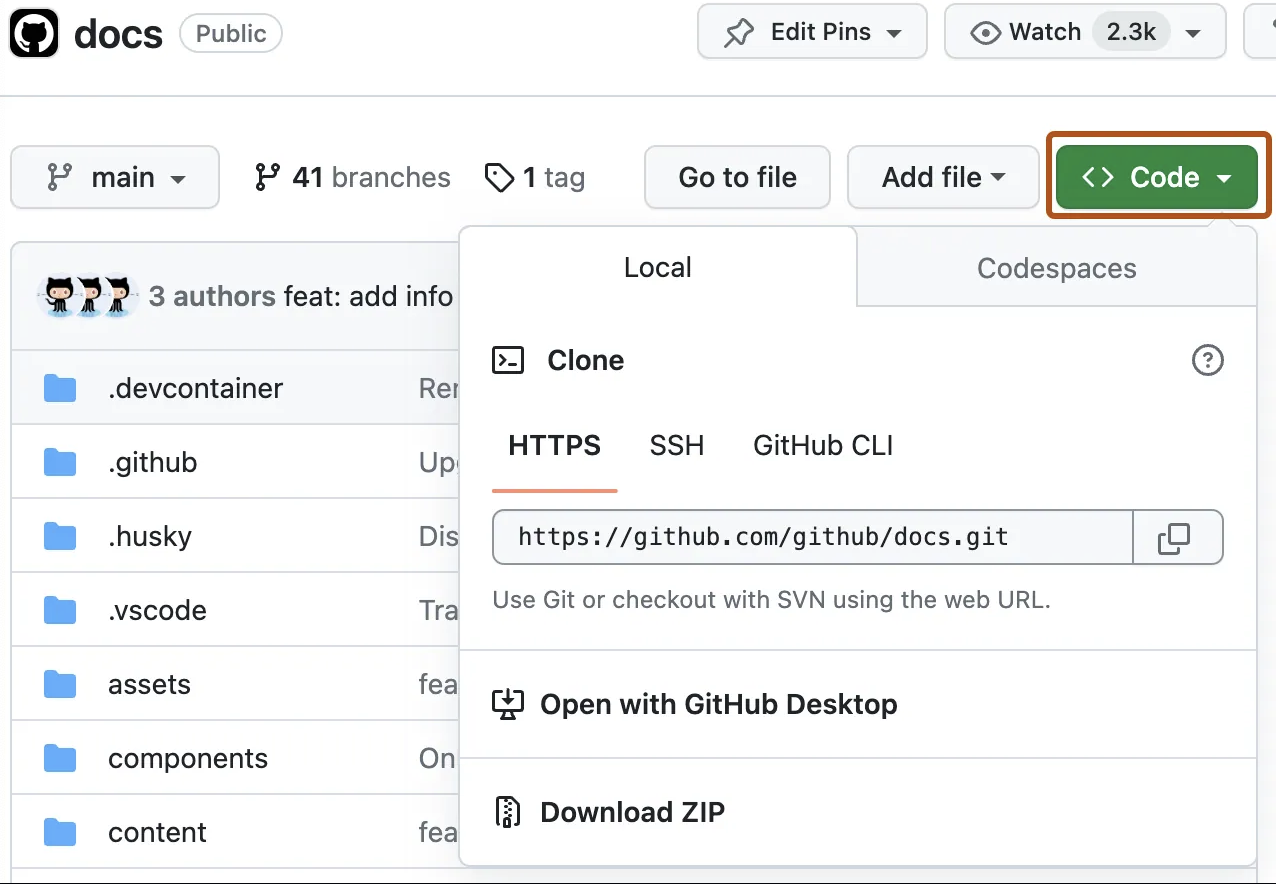
\includegraphics[width=0.8\textwidth]{assets/fig1.png}
\end{figure}

When you run \texttt{git clone}, the following actions occur: 
\begin{itemize}
    \item A new folder called \texttt{repo} is made
    \item It is initialized as a Git repository
    \item A remote named \texttt{origin} is created, pointing to the URL you cloned from  
    \item All of the repository's files and commits are downloaded there 
    \item The default branch is checked out 
\end{itemize}

For every branch \texttt{foo}, a corresponding remote-tracking branch \texttt{refs/remotes/origin/foo} is created in your local repository. You can usually abbreviate such remote-tracking branch names to \texttt{origin/foo}.

\subsection{Fetching changes from a remote repository}

Use \texttt{fit fetch} to retrieve new work done by other people. Fetching from a repository grabs all the new remote-tracking branches and tags without merging those changes into your own branches.

If you already have a local repository with a remote URL set up for the desired project, you can grab all the new information by using \texttt{fit fetch *remotename*} in the terminal.

\begin{codeblock}[language=bash]
git fetch REMOTE-NAME 
# Fetches updates made to a remote repository 
\end{codeblock}

\subsection{Merging changes into your local branch}

Merging combines your local changes with changes made by others.

Typically, you'd merge a remote-tracking branch (i.e., a branch fetched from a remote repository) with your local branch:
\begin{codeblock}[language=bash]
git merge REMOTE-NAME/BRANCH-NAME 
# Merges updates made online with your local work 
\end{codeblock}

\subsection{Pulling changes from a remote repository}

\texttt{git pull} is a convenient shortcut for completing both \texttt{git fetch} and \texttt{git merge} in the same command:
\begin{codeblock}[language=bash]
git pull REMOTE-NAME BRANCH-NAME 
# Grabs online updates and merges them with your local work 
\end{codeblock}

Because \texttt{pull} performs a merge on the retrieved changes, you should ensure that your local work is committed before running the \texttt{pull} command. If you run into a \textbf{merge conflict} you cannot resolve, or if you decide to quit the merge, you can use \texttt{git merge --abort} to take the branch back to where it was in before you pulled. 


\newpage
\section{Dealing with non-fast-forward errors}

Sometimes, Git can't make your change to a remote repository without losing commits. When this happens, your push is refused. 

If another person has pushed to the same branch as you, Git won't be able to push your changes:
\begin{exampleblock}
    \begin{codeblock}[language=bash]
git push origin main
> To https://github.com/USERNAME/REPOSITORY.git
>  ! [rejected]        main -> main (non-fast-forward)
> error: failed to push some refs to 'https://github.com/USERNAME/REPOSITORY.git'
> To prevent you from losing history, non-fast-forward updates were rejected
> Merge the remote changes (e.g. 'git pull') before pushing again. See the
> 'Note about fast-forwards' section of 'git push --help' for details.
    \end{codeblock}
\end{exampleblock}

You can fix this by fetching and merging the changes made on the remote branch with the changes that you have made locally:
\begin{codeblock}[language=bash]
git fetch origin 
# Fetches updates made to an online repository

git merge origin YOUR_BRANCH_NAME
# Merges updates made online with your local work
\end{codeblock}

Or simply use \texttt{git pull} to perform both commands at once:
\begin{codeblock}[language=bash]
git pull origin YOUR_BRANCH_NAME 
# Grabs online updates and merges them with your local work 
\end{codeblock}